% =====================================================================
%  Презентация к проекту «Экономические убытки сельского хозяйства от засух»
%  Компиляция: pdfLaTeX (Overleaf).
% =====================================================================
\documentclass[aspectratio=169,11pt]{beamer}
\usepackage[T2A]{fontenc}
\usepackage[utf8]{inputenc}
\usepackage[english,russian]{babel}
\usepackage{graphicx}
\graphicspath{{figures/}}
\usepackage{booktabs}

\usetheme{Madrid}
\usecolortheme{whale}
\setbeamertemplate{navigation symbols}{}
\setbeamertemplate{caption}{\insertcaption}
\setbeamerfont{title}{size=\large}
\setbeamertemplate{footline}[frame number]

\title[Засухи и убытки АПК]{Экономические убытки сельского хозяйства от засух}
\subtitle{Оценка по индексам засушливости и данным об урожайности}
\author{Студенческий проект, НИУ ВШЭ}
\date{2026}

\begin{document}

\begin{frame}[plain]\titlepage\end{frame}

% ---------------------------------------------------------------
\begin{frame}{Проблема и актуальность}
\begin{itemize}
  \item Негативные природные явления (засухи, жара, заморозки, наводнения, пожары) наносят АПК большой экономический ущерб.
  \item \textbf{Засуха}: природное явление, наиболее тяжело сказывающееся на сельском хозяйстве (ФАО, 2021).
  \item Россия: крупный производитель и экспортёр зерна; засухи 2010 и 2012 гг. вызвали обвал сбора, рост цен и запрет экспорта.
  \item Частота и интенсивность засух растут при потеплении $\Rightarrow$ нужна количественная оценка климатических рисков.
\end{itemize}
\end{frame}

% ---------------------------------------------------------------
\begin{frame}{Цель и задачи}
\textbf{Цель:} количественно оценить влияние засух на урожайность зерновых и связанные экономические потери на реальных открытых данных.
\medskip
\begin{enumerate}
  \item обзор литературы (НПЯ, индексы засухи, методы);
  \item сбор данных и расчёт индексов SPI / SPEI;
  \item оценка связи: корреляции $\to$ панель $\to$ машинное обучение;
  \item денежная оценка убытков;
  \item код и отчёт.
\end{enumerate}
\end{frame}

% ---------------------------------------------------------------
\begin{frame}{Что известно из литературы}
\begin{itemize}
  \item \textbf{Индексы засухи:} SPI (осадки) $\to$ SPEI (осадки $-$ испаряемость), чувствительный к жаре.
  \item \textbf{Глобально:} засухи снижают сбор зерновых на $\sim$9--10\% (Lesk, 2016); климат объясняет $\sim$1/3 изменчивости урожая (Ray, 2015).
  \item \textbf{Методы:} случайный лес точнее линейной регрессии (Jeong, 2016); панельные модели для России (Belyaeva \& Bokusheva, 2018).
  \item \textbf{Россия:} засуха 2010 года снизила сбор зерна с $\sim$97 до $\sim$61 млн т (Wegren, 2011).
\end{itemize}
\centerline{\footnotesize Всего в списке литературы 28 источников.}
\end{frame}

% ---------------------------------------------------------------
\begin{frame}{Постановка задачи}
\begin{itemize}
  \item \textbf{Главный кейс: Россия};\ для мощности и робастности добавлены страны зернового пояса: Украина, Казахстан, Беларусь, Молдова, Румыния.
  \item Аномалия урожая: отклонение от технологического тренда (LOESS), \%.
  \item Засушливость $D$: SPEI/SPI, аномалии температуры и осадков лета, ONI.
  \item Гипотеза: $\partial a/\partial \text{SPEI}>0$, $\partial a/\partial T_{\text{лето}}<0$.
  \item Убытки: $L=\sum_c \max(0,\hat y_c-y_c)\cdot A_c \cdot p_c$.
\end{itemize}
\end{frame}

% ---------------------------------------------------------------
\begin{frame}{Данные и методы}
\textbf{Данные (открытые, реальные):}
\begin{itemize}
  \item FAOSTAT: урожайность, площади, сбор, цены (1992--2024);
  \item World Bank CCKP: осадки и температура, CRU TS 4.07 (1901--2022);
  \item NOAA ONI: индекс Эль-Ниньо (ENSO).
\end{itemize}
\textbf{Методы:} собственный расчёт SPI/SPEI (Торнтвейт + лог-логистика) $\to$ корреляции $\to$ панель FE (\texttt{PanelOLS}) $\to$ ML (CatBoost, RF) $\to$ денежные убытки. Полностью воспроизводимо: \texttt{python src/run\_all.py}.
\end{frame}

% ---------------------------------------------------------------
\begin{frame}{Результат 1. Урожай и засухи}
\begin{columns}
\column{0.5\textwidth}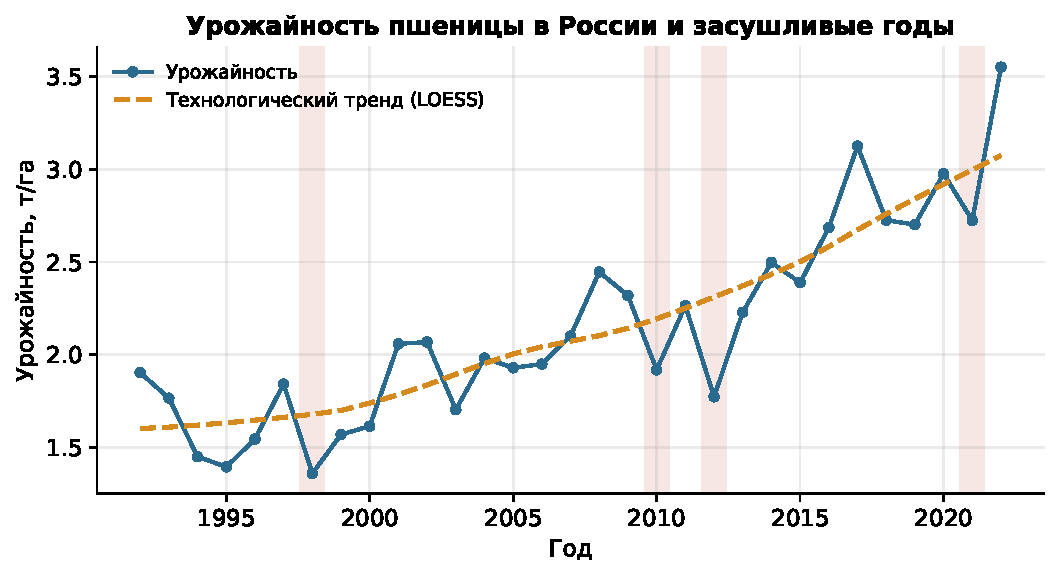
\includegraphics[width=\linewidth]{fig01_russia_yield_trend.pdf}
\column{0.5\textwidth}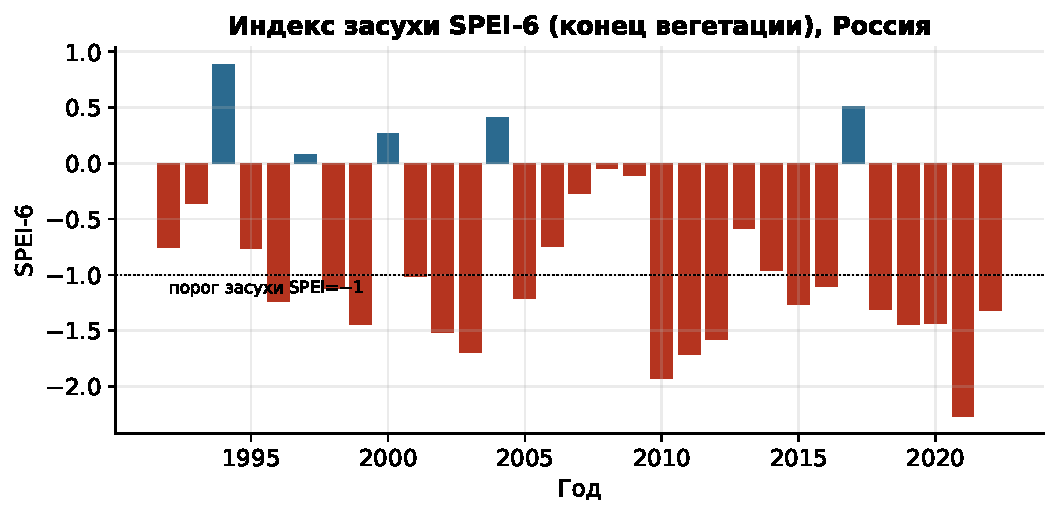
\includegraphics[width=\linewidth]{fig04_russia_spei_timeseries.pdf}
\end{columns}
\centerline{\footnotesize Провалы урожая 2010 и 2012 гг. совпадают с отрицательными SPEI.}
\end{frame}

% ---------------------------------------------------------------
\begin{frame}{Результат 2. Корреляции}
\begin{columns}
\column{0.46\textwidth}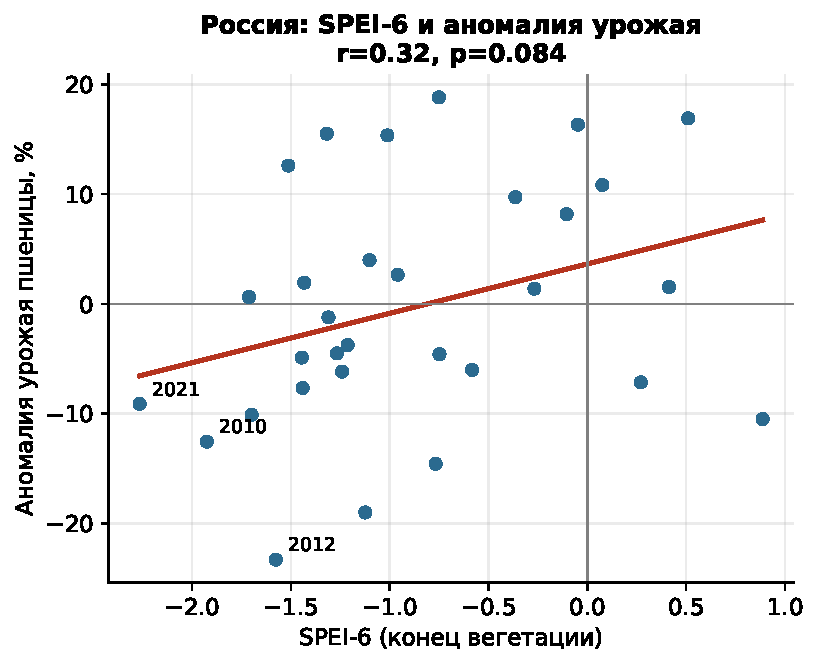
\includegraphics[width=\linewidth]{fig02_russia_spei_yield_scatter.pdf}
\column{0.54\textwidth}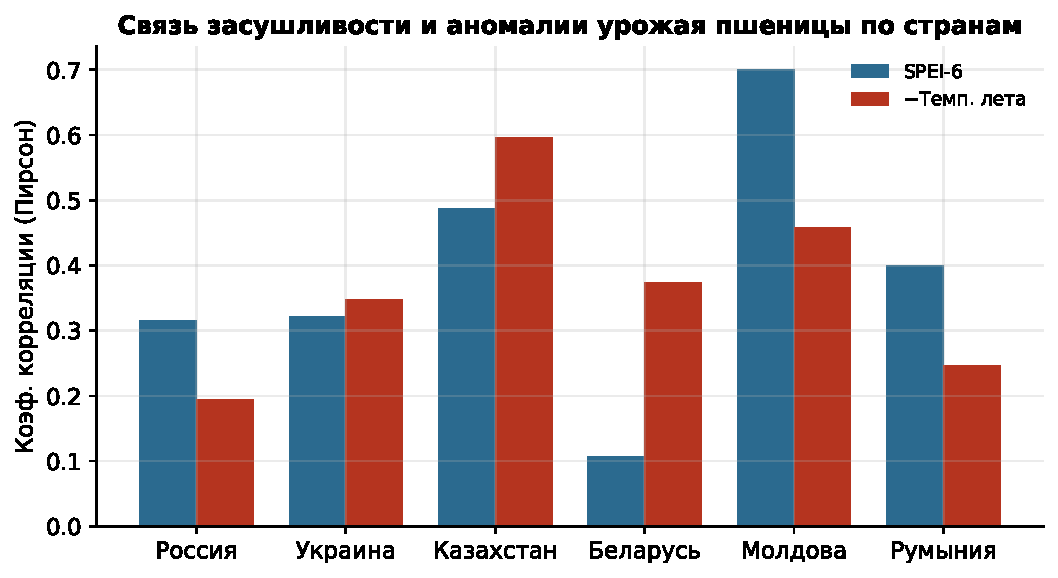
\includegraphics[width=\linewidth]{fig03_country_corr_bars.pdf}
\end{columns}
\centerline{\footnotesize Панель с FE: SPEI-6 $r=0{,}42$ ($p<0{,}001$). В степных странах связь сильнее, во влажной Беларуси слабее.}
\end{frame}

% ---------------------------------------------------------------
\begin{frame}{Результат 3. Панельные регрессии}
\centering
\small
\begin{tabular}{lccc}
\toprule
 & (A) Пшеница & (B) Все культуры & (C) +годы \\
\midrule
SPEI-6 & $5{,}49^{***}$ & $5{,}71^{***}$ & $4{,}27$ \\
Темп. лета (z) & $-2{,}32$ & $-0{,}47$ & $-7{,}46^{*}$ \\
ONI лето & $3{,}64^{**}$ & $2{,}57$ & --- \\
\midrule
$R^2$ внутр. & 0{,}21 & 0{,}12 & 0{,}14 \\
\bottomrule
\end{tabular}
\medskip
\begin{itemize}\footnotesize
  \item +1$\sigma$ SPEI $\Rightarrow$ +4--6\% к урожаю; экстремальная жара $\Rightarrow$ $-7{,}5$\%.
\end{itemize}
\end{frame}

% ---------------------------------------------------------------
\begin{frame}{Результат 4. Машинное обучение}
\begin{columns}
\column{0.5\textwidth}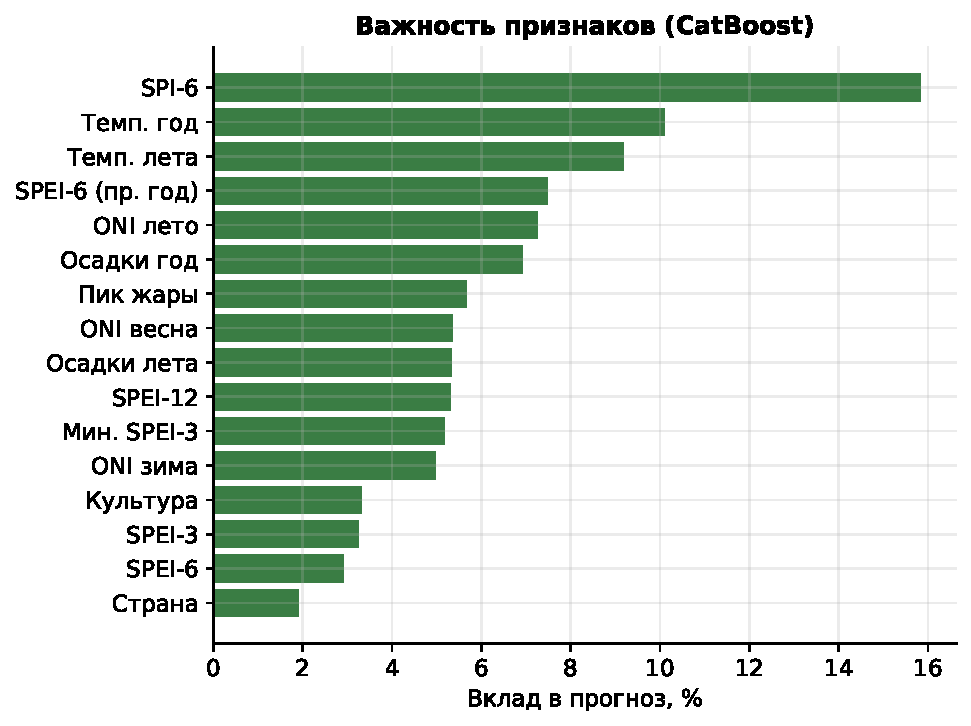
\includegraphics[width=\linewidth]{fig05_feature_importance.pdf}
\column{0.5\textwidth}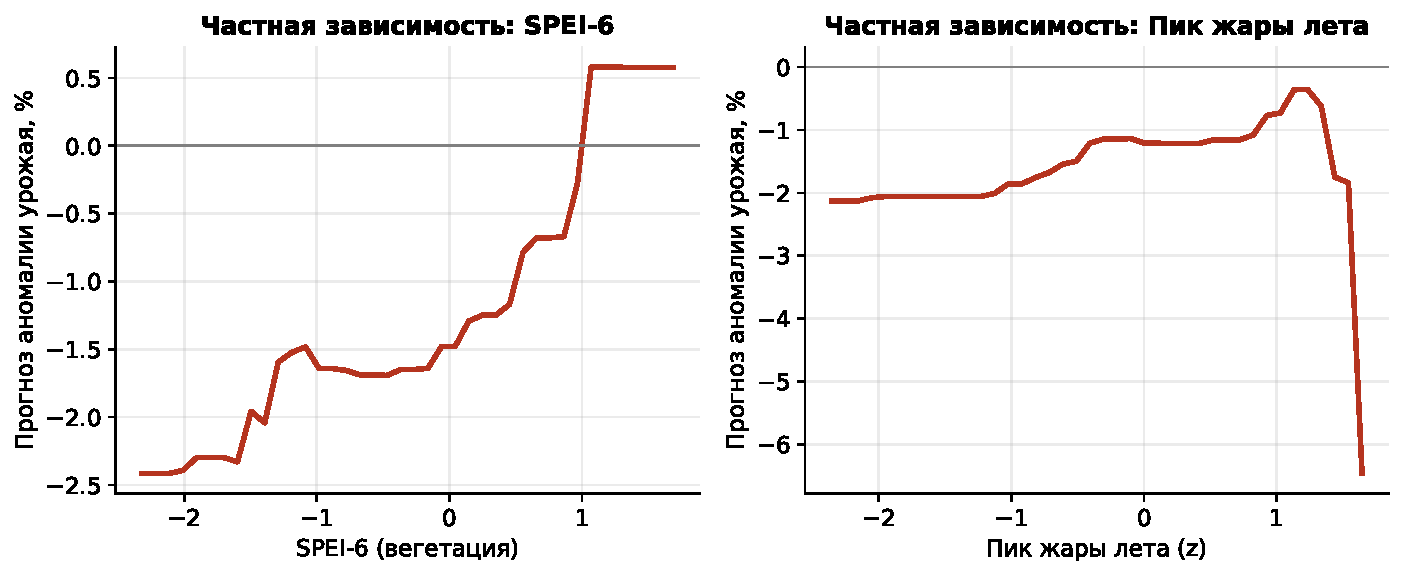
\includegraphics[width=\linewidth]{fig06_partial_dependence.pdf}
\end{columns}
\centerline{\footnotesize Станд. CV: CatBoost/RF $R^2\approx0{,}37$ (vs 0{,}19 у OLS); строгая CV по годам: $\approx0{,}07$. Связи физичны.}
\end{frame}

% ---------------------------------------------------------------
\begin{frame}{Результат 5. Экономические убытки}
\centering
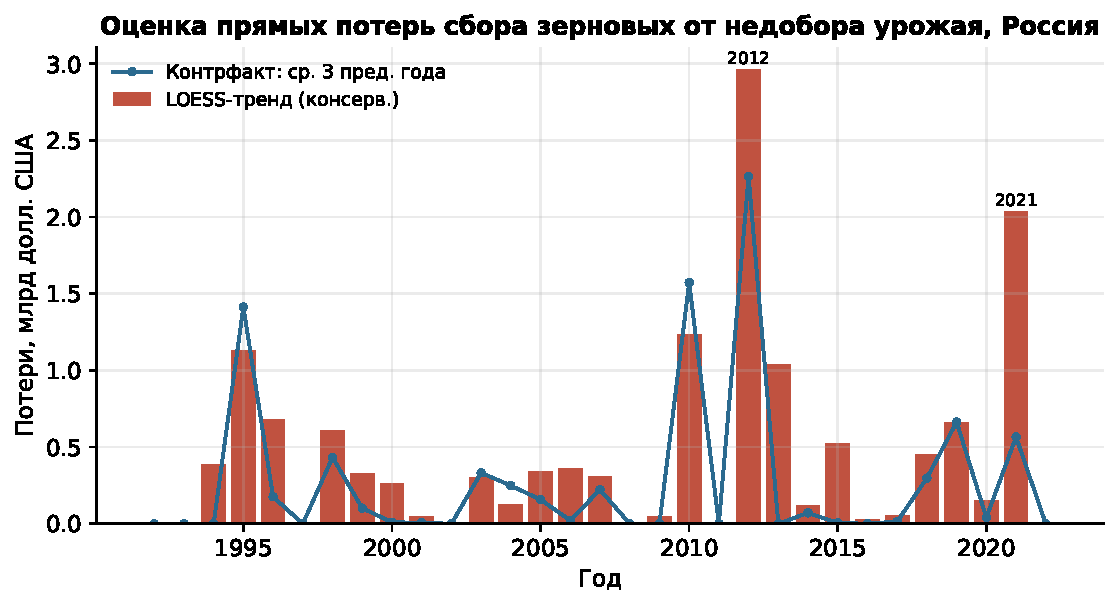
\includegraphics[width=0.74\textwidth]{fig08_economic_loss.pdf}
\begin{itemize}\footnotesize
  \item 2012: $\sim$3{,}0 млрд \$ ($-$18\%); 2010: $\sim$1{,}2 млрд \$; 2021: $\sim$2{,}0 млрд \$.
  \item Накопленно 2000--2022: $\sim$6{,}5--11 млрд \$ (диапазон по контрфактам; без косвенных потерь).
\end{itemize}
\end{frame}

% ---------------------------------------------------------------
\begin{frame}{Ограничения и план усложнения}
\textbf{Ограничение снято на стороне климата:} пересчёт по \emph{зерновому поясу} (сетка GPCC + GHCN-CAMS) усиливает связь: корреляция с жарой $0{,}26\to0{,}48$, SPEI засухи-2010 $-1{,}9\to-2{,}6$ (рис. в отчёте).
\medskip
\textbf{Дальше:}
\begin{enumerate}
  \item субнациональный уровень (регионы + климат зерновых районов);
  \item фенология и культуроспецифичные окна вегетации;
  \item данные дистанционного зондирования (NDVI, влажность почвы);
  \item имитационное моделирование (AquaCrop) и климатические сценарии.
\end{enumerate}
\end{frame}

% ---------------------------------------------------------------
\begin{frame}{Выводы}
\begin{itemize}
  \item Засушливость \textbf{значимо} связана с урожаем: SPEI-6 $r=0{,}42$ ($p<0{,}001$); +1$\sigma$ SPEI $\Rightarrow$ +4--6\%, жара $\Rightarrow$ $-7$\%.
  \item ML: $\sim$37\% дисперсии (станд. CV) против 7\% на новых годах; изменчивость в основном неклиматическая.
  \item Прямые потери зерна в засухи: 1--3 млрд \$/год, до 18\% стоимости.
  \item Всё на \textbf{реальных открытых данных}, код воспроизводим.
\end{itemize}
\end{frame}

% ---------------------------------------------------------------
\begin{frame}[plain]
\centering
\vfill
{\Large Спасибо за внимание!}\\[4mm]
{\footnotesize Код и данные: \texttt{github.com/moura27272727-pixel/agro-drought-losses}}
\vfill
\end{frame}

\end{document}
